\documentclass[]{article}

% Imported Packages
%------------------------------------------------------------------------------
\usepackage{amssymb}
\usepackage{amstext}
\usepackage{amsthm}
\usepackage{amsmath}
\usepackage{enumerate}
\usepackage{fancyhdr}
\usepackage[margin=1in]{geometry}
\usepackage{graphicx}
\usepackage{extarrows}
\usepackage{setspace}
\usepackage{graphicx}
\graphicspath{ {./asset/} }
%\usepackage{extarrows}
%\usepackage{setspace}
%\usepackage{xcolor}
\usepackage{color}
%------------------------------------------------------------------------------

% Header and Footer
%------------------------------------------------------------------------------
\pagestyle{plain}  
\renewcommand\headrulewidth{0.4pt}                                      
\renewcommand\footrulewidth{0.4pt}                                    
%------------------------------------------------------------------------------

% Title Details
%------------------------------------------------------------------------------
\title{Deliverable \#1 Software Requirement Specification (SRS)}
\author{SE 3A04: Software Design II -- Large System Design}
\date{}                              
%------------------------------------------------------------------------------

% Document
%------------------------------------------------------------------------------
\begin{document}

\maketitle	
\noindent{\bf Tutorial Number:} T01\\
{\bf Group Number:} G6 \\
{\bf Group Members:} 
\begin{itemize}
	\item Jane Klavir
	\item Nathan Luong
	\item Areez Visram
	\item Jennifer Ye
\end{itemize}

\section{Introduction}
\label{sec:introduction}
% Begin Section

The following document is dedicated to showcasing the requirements of the taxi carpool app requested by a local taxi company. The app is dedicated to make rides cheaper and more convenient for their riders. This app is also meant to be a long-term project for the company, meaning this \textbf{SRS} is a living document which has the possibility of changing in the future. This document will explain the important stakeholders involved, requirements and viewpoints of each while also explaining the main functions of the app.

\subsection{Purpose}
\label{sub:purpose}
% Begin SubSection
This \textbf{SRS} is meant for developers, stakeholders and direct players in the planning and development of the app and should be understandable for all those involved. This \textbf{SRS} will further break down the functionalities, constraints, use cases and overall design of the project in further detail. 

% End SubSection

\subsection{Scope}
\label{sub:scope}
% Begin SubSection
To develop this project the production of the main taxi request and offer app called TaxiCarPool, the Conversation Prompt Generator and a variety of databases will have to be produced. There will not be a need to produce a payment system into the app as this will be handled by the taxi company payment systems. The project will only project the cost of the ride but will not handle the payments as it is not part of the app’s main functionality.
\newline \newline
The TaxiCarPool app will perform the main functions of the app. This will include allowing users to request a carpool taxi, receive a list of possible rides to select and allow current rides to allow carpooling in their car. This product’s objective is to perform the main functions of matchmaking users to a carpool to save money. 
\newline \newline
The Conversation Prompt Generator will randomly generate a conversation starter for the riders to use based on their profile. Their profile will specify if they want to use this feature and if so, what they are interested in. The generator will not be forced upon any of the users and can be switched off if desired. The goal of this product is to create a friendly environment when carpooling with others that one may not know. This function is mostly dedicated to benefit those who are carpooling to a further distance.
\newline \newline
The creation of a database will hold all the necessary information for the app to function, making it easily accessible and manageable. The information being stored can range from user information; name, email, phone number, to riding history, to preferences of taxi times, models, or other passengers. 
% End SubSection

\subsection{Definitions, Acronyms, and Abbreviations}
\label{sub:definitions_acronyms_and_abbreviations}
% Begin SubSection
BE: Business Event is something that occurs between the client/stakeholder and the system. 
\newline \newline
SRS: Software Requirements Specification is a document that explains the requirements of the software being developed.
\newline \newline
VP: Viewpoint, often in reference to a stakeholder/client interested in the system and how they view the business event. \\ \\
CF: Creative Feature, an indication to one of the creative/innovative features
% End SubSection

\subsection{References}
\label{sub:references}
% Begin SubSection
\begin{itemize}
	\item Johns, K. (2022, July 7). Why design is the most important factor in a mobile app development?: ISHIR- mobile application development company india. ISHIR. Retrieved February 11, 2023, from https://www.ishir.com/blog/9633/why-design-is-the-most-important-factor-in-a-mobile-app-development.htm 
	\item Office of the Privacy Commissioner of Canada. (2018, January 31). Summary of privacy laws in Canada. Office of the Privacy Commissioner of Canada. Retrieved February 25, 2023, from https://www.priv.gc.ca/en/privacy-topics/privacy-laws-in-canada/02-05-d-15/heading-0-0-2-1
	\item Schoenfelder, N. (n.d.). What are good latency \& ping speeds? Graphical Network Monitoring and Troubleshooting. Retrieved February 11, 2023, from https://www.pingplotter.com/wisdom/article/is-my-connection-good 
	\item statcounter. (n.d.). Mobile Operating System Market Share Worldwide. StatCounter Global Stats. Retrieved February 11, 2023, from https://gs.statcounter.com/os-market-share/mobile/worldwide 
	\item UGEM. (2020, June 15). What are the core features of Minimalist app design? UGEM. Retrieved February 11, 2023, from https://ugem.design/blog/minimal-app-design 
\end{itemize}
% End SubSection

\subsection{Overview}
\label{sub:overview}
% Begin SubSection
This \textbf{SRS} is structured to first give background information about the app. This will include how the app will interface with the taxi companies, along with the general functionalities and assumptions that are being made. The document will then follow with showcasing one of the main business events and its related use cases. This will explain how the main function will work across different scenarios and stakeholders in a visual manner. This will be further expanded upon in more detail throughout the document. It will include more business events with a variety of viewpoints and scenarios for both the function shown in the use case diagram and other main function of the project. This document will conclude by explaining the non-functional requirements involving presentation, performance, usability, security, and maintainability notes of the project.
% End SubSection

% End Section

\section{Overall Description}
\label{sec:overall_description}
% Begin Section


\subsection{Product Perspective}
\label{sub:product_perspective}
% Begin SubSection

	The product being developed is an Android application which empowers the ability to book carpools via a user-friendly interface. The application will securely store customer personal information such as carpool request histories, and personal data inputted by the user. The product is not self-contained since its functionality depends on Google Maps for mapping integration. The product scope mainly covers a match making functionality to match potential carpoolers together. The feature will be implemented under a centralized dispatcher which communicate with the mobile app and user’s database. Fare determination will be covered under the scope of the app, however payment processing is external to the system. The general interaction can be visualized as follows: 
	\begin{center}
		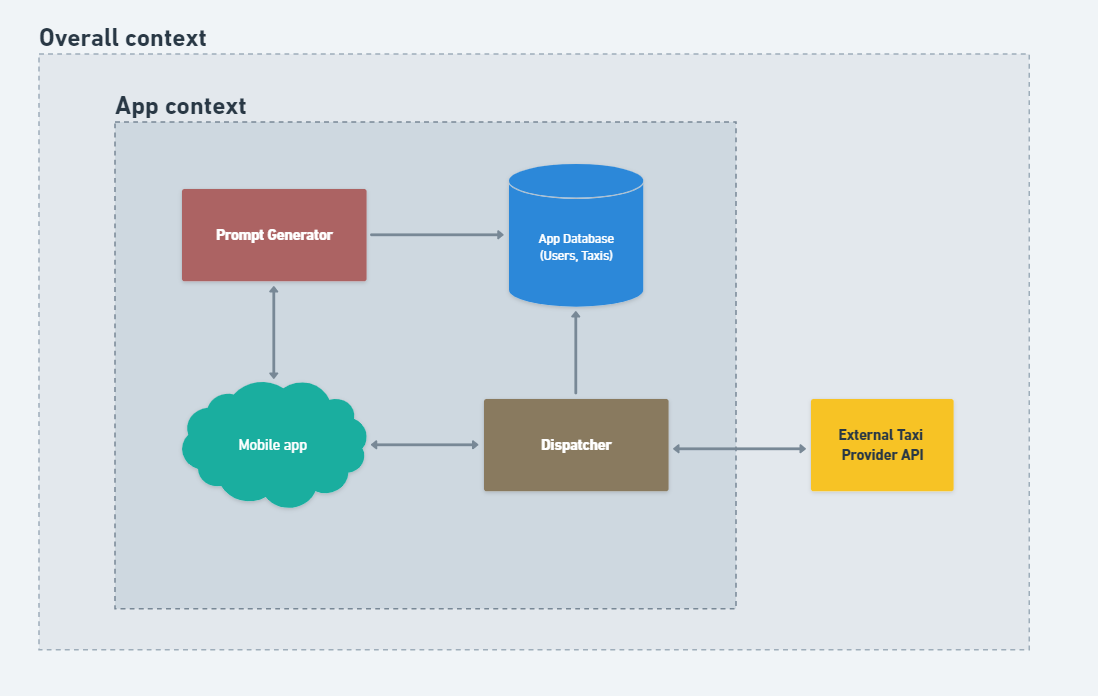
\includegraphics[scale=0.7]{app-context.png}
	\end{center}


% End SubSection

\subsection{Product Functions}
\label{sub:product_functions}
% Begin SubSection
	\begin{center}
		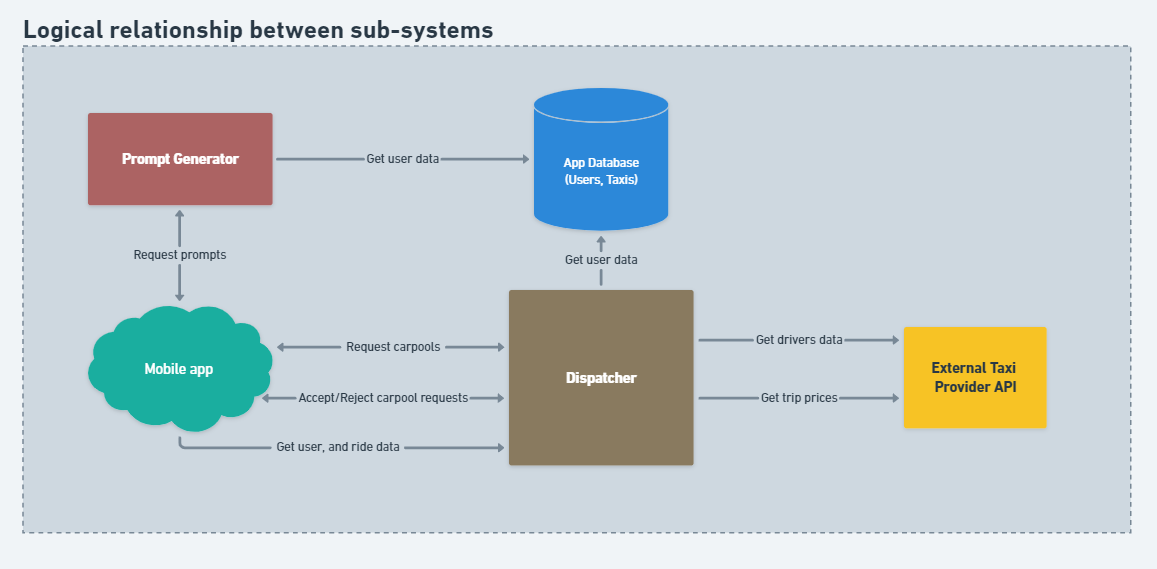
\includegraphics[scale=0.7]{subsys-relationship.png}
	\end{center}

\begin{enumerate}[a)]
	\item \textbf{User registration and profile editing: }Users can register to use the taxi service and later can edit or remove their information.
	\item \textbf{Requesting taxi: }Users can enter search criteria to request a taxi. Based on the user’s profile, the app will return a list of best-fit matches. Users choose the desired match and other carpooler will be notified. 
	\item \textbf{Reviewing offer: }The app displays offers information to the users to choose between.
	\item \textbf{Taxi check-in: }Users can scan or enter the taxi ID when it arrives to check in and use the service.
	\item \textbf{Fare calculation and display:  }Trip prices are calculated, using a fixed rate per kilometer, and presented to the users before reaching their destination. 
	\item \textbf{Google Maps Integration:  }The app interface will use Google Maps to visualize pick-up, drop-off loacation. 
	\item \textbf{Data encryption:  }The software system will encrypt all messages when transmitting. Important information like password or user’s postal code will also be encrypted when storing within the database.
	\item \textbf{Trips rating:  }After each trip, users can enter their rating to help improving the service.
	\item \textbf{Prompts Generation:  }Users of the taxi service can engage in a prompt-based game while carpooling. When the users activate prompts, the app will return a list of personalized prompts for carpoolers to engage with when they are on the same car.


\end{enumerate}

% End SubSection

\subsection{User Characteristics}
\label{sub:user_characteristics}
% Begin SubSection

\begin{enumerate}[a)]
	\item Riders should be comfortable with using Android mobile devices.
	\item Riders might be sensitive with prices and therefore opt for carpools instead of regular taxi services.
	\item Riders might be outgoing, socially engaged, and interested in meeting new people.
	\item Riders are most likely live in a big city since taxi services are highly available, and parking fees are expensive.
	\item Riders might have a busy schedule since taking public transport or maintaining their own car takes time and effort.



\end{enumerate}

% End SubSection

\subsection{Constraints}
\label{sub:constraints}
% Begin SubSection
\begin{enumerate}[a)]
	\item \textbf{Geographical:} The app can only operate in Canada.
	\item \textbf{Internet:} The app functionality relies heavily on the internet to book, checkin, and view taxi’s location.
	\item \textbf{Taxi Regulation:} Since the app is working in conjunction with the taxi provider, it must follow taxi law and regulation. For example, the fare structure used by the app must be approved by the Board of Transportation for some cities.
	\item \textbf{Data Privacy Regulation:} Personal data stored within the app needs to be encrypted and processed in a way that complies with the Canadian Personal Information Protection and Electronic Documents Act.
	\item \textbf{Technological:} Since the app is dependent on Google Maps, it can not extend to provide a better mapping experience than what Google Maps offers. 

\end{enumerate}

% End SubSection

\subsection{Assumptions and Dependencies}
\label{sub:assumptions_and_dependencies}
% Begin SubSection


\begin{enumerate}[a)]
	\item Assumptions

	\begin{itemize}
		\item Users have an android mobile device. If users use IOS or other operating system, the app would not be available.
		\item Users have a highly available internet connection. The app will not function when internet connection is not present.
		\item Drivers information are provided and available via the app\textquotesingle s database. If the assumption does not hold, driver's data will be pulled from an external data source.
		\item Prices are determined via a fixed rate per kilometer.
		\item Payment processing is external and not under the scope of the application. If the assumption does not hold, an integration with external Payment Service Provider need to be implemented.
	\end{itemize}

\end{enumerate}
% End SubSection

\subsection{Apportioning of Requirements}
\label{sub:apportioning_of_requirements}
% Begin SubSection

\begin{enumerate}[a)]
	\item Real-time trip tracking via Google Maps Interface.
	\item Accurate personalized prompts based on user trip history, behaviour, and more. 
\end{enumerate}

% End SubSection

% End Section
\section{Use Case Diagram}
\label{sec:use_case_diagram}
% Begin Section
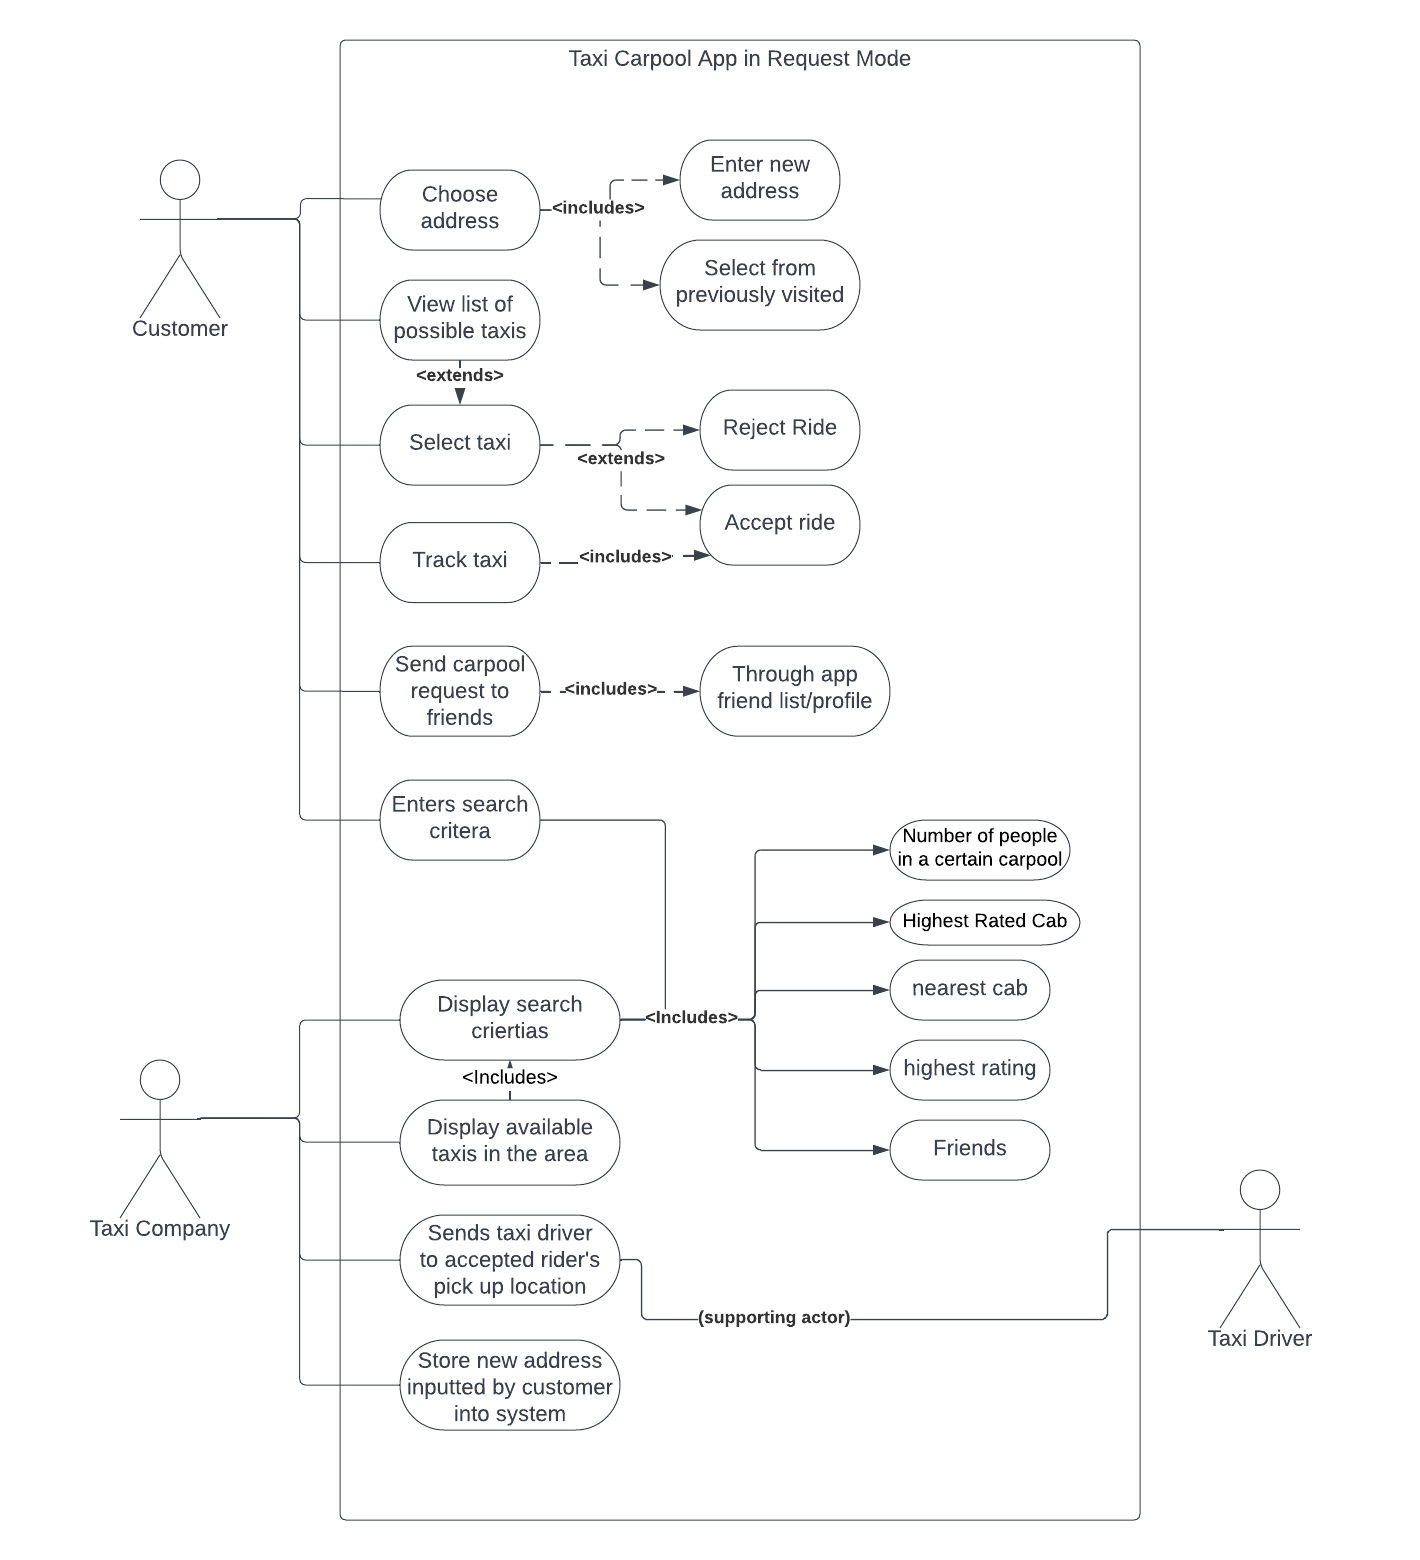
\includegraphics[scale = 0.8]{Use_Case_Diagram.png}
% End Section

\newpage
\section{Functional Requirements}
\label{sec:functional_requirements}
% Begin Section

Note: Requirements in blue are ``extra'' and can be ignored in initial design stages\\

\begin{enumerate}[{\textbf{BE}}1.]
    \item Customer creates new user profile
    \begin{enumerate}[{\textbf{VP}1}.1]
        \item Customers
            \begin{enumerate}
                \item[$S_1$] System asks for customer’s information
                \item[$E_1$] Customer inputs their information
                \begin{enumerate}
                    \item[$S_{1.1}$] Certain information must be unique
                \end{enumerate}
\color{blue}
                \item[$S_2$] System asks customer to verify email or phone number
                \item[$E_2$] Customer verifies email or phone number
\color{black}
                \item[$S_3$] System stores customer profile in database
            \end{enumerate}
        \item Taxi company
            \begin{enumerate}
                \item[N/A]
            \end{enumerate}
        \item Taxi drivers
            \begin{enumerate}
                \item[N/A]
            \end{enumerate}
        \item Investors
            \begin{enumerate}
	       \color{blue}
                \item[$S_1$] Every new 1000 sign-ups, system sends notification to investors
                \color{black}
            \end{enumerate}
        \item Legal
            \begin{enumerate}
                \item[$S_1$] System securely stores user data to comply with GDPR privacy
            \end{enumerate}
        \item[Global] Scenario for \textbf{BE}1
            \begin{enumerate}
                \item[$S_1$] System asks for customer’s information
                \item[$E_1$] Customer inputs their information in all mandatory fields
                \begin{enumerate}
                \item[$E_{1.1}$] Certain information must be unique
                \end{enumerate}
\color{blue}
                \item[$S_2$] System asks customer to verify email or phone number
                \item[$E_2$] Customer verifies email or phone number
\color{black}
                \item[$S_3$] System registers customer profile as user in system
                \begin{enumerate}
                \item[$S_{3.1}$] System securely stores user data to comply with GDPR privacy
\color{blue}
                \item[$S_{3.2}$] Every new 1000 sign-ups, system sends notification to investors
\color{black}
                \end{enumerate}
            \end{enumerate}
    \end{enumerate}
    \item Customer edits their profile
    \begin{enumerate}[{\textbf{VP2}}.1]
        \item Customers
            \begin{enumerate}
                \item[$S_1$] System asks customer to authenticate themselves
                    \item[$E_1$] Customer completes authentication process
                \item[S2] System displays user profile
                \begin{enumerate}
                    \item[$E_{2.1}$] Customer edits information
                    \item[$E_{2.2}$] Customer saves edits, given that all mandatory information is entered
                \end{enumerate}
                \item[$S_3$] System saves user profile
            \end{enumerate}
        \item Taxi company
            \begin{enumerate}
                \item[N/A]
            \end{enumerate}
        \item Taxi drivers
            \begin{enumerate}
                \item[N/A]
            \end{enumerate}
        \item Investors
            \begin{enumerate}
                \item[N/A]
            \end{enumerate}
        \item Legal
            \begin{enumerate}
                \item[$S_1$] System securely stores user data to comply with GDPR privacy
            \end{enumerate}
        \item[Global] Scenario for \textbf{BE}2
            \begin{enumerate}
                \item[$S_1$] System asks customer to authenticate themselves
                    \item[$E_1$] Customer completes authentication process
                \item[$S_2$] System displays user profile
                \begin{enumerate}
                    \item[$E_{2.1}$] Customer edits desired information
                    \item[$E_{2.2}$] Customer saves edits, given that all mandatory information is entered
                \end{enumerate}
                \item[$S_3$] System saves user profile
                \begin{enumerate}
                    \item[$S_{3.1}$] System securely stores user data to comply with GDPR privacy
                \end{enumerate}
            \end{enumerate}
    \end{enumerate}


\item Customer deletes their profile
    \begin{enumerate}[{\textbf{VP3}}.1]
        \item Customers
            \begin{enumerate}
                  	 \item[$S_1$] System asks customer to authenticate themselves	
                   	 \item[$E_1$] Customer completes authentication process
			\item[$S_2$] System asks customer to confirm they want to delete their account
                   \item[$E_2$] Customer confirms they want to delete their account
\color{blue}
                \item[$S_3$] System asks customer to verify email or phone number
                \item[$E_3$] Customer verifies email or phone number
\color{black}
                \item[$S_4$] Customer profile removed from database
            \end{enumerate}
        \item Taxi company
            \begin{enumerate}
                \item[$S_1$] 
            \end{enumerate}
        \item Taxi drivers
            \begin{enumerate}
                \item[N/A]
            \end{enumerate}
        \item Investors
            \begin{enumerate}
                \item[N/A]
            \end{enumerate}
        \item Legal
            \begin{enumerate}
                \item[$S_1$] System removes all user data to comply with GDPR privacy
            \end{enumerate}
        \item[Global] Scenario for \textbf{BE}3
            \begin{enumerate}
                  	 \item[$S_1$] System asks customer to authenticate themselves	
                   	 \item[$E_1$] Customer completes authentication process
			\item[$S_2$] System asks customer to confirm they want to delete their account
                   \item[$E_2$] Customer confirms they want to delete their account
\color{blue}
                \item[$S_3$] System asks customer to verify email or phone number
                \item[$E_3$] Customer verifies email or phone number
\color{black}
                \item[$S_4$] Customer profile removed from database
\begin{enumerate}
		\item[$S_{4.1}$] System removes all user data to comply with GDPR privacy
\end{enumerate}
            \end{enumerate}
    \end{enumerate}


    \item Taxi carpool is requested
    \begin{enumerate}[{\textbf{VP4}}.1]
        \item Customers
            \begin{enumerate}
                \item[$S_1$] System asks customer to input their destination
                \item[$E_1$] Customer inputs destination
	     \item[$S_2$] System asks customers to enter search criteria
	     \item[$E_2$] Customer inputs search criteria
 	     \item[$S_3$] System returns best matches
                \item[$E_3$] Customer selects taxi to send their carpool request to
\item[$S_{4.1}$] System sends customer's request to carpool offerer
                \begin{enumerate}
                    \item[$S_{4.2}$] Customers are returned to selection phase (i.e. after inputting destination) if request is denied, branch to S2
                    \item[$S_{4.3}$] Customers notified if request is accepted
                \end{enumerate}
                \item[$S_5$] System shows location of designated cab
            \end{enumerate}
        \item Taxi company
            \begin{enumerate}
                \item[$S_1$] System computes estimated payment split based on taxi company's fares
	        \item[$S_2$] System notifies taxi company of new carpool
            \end{enumerate}
        \item Taxi drivers
            \begin{enumerate}
                \item[N/A]
            \end{enumerate}
        \item Investors
            \begin{enumerate}
                \item[N/A]
            \end{enumerate}
        \item Legal
            \begin{enumerate}
                \item[N/A]
            \end{enumerate}
        \item[Global] Scenario for \textbf{BE}4
            \begin{enumerate}
                \item[$S_1$] System asks customers to input their destination
                \item[$E_1$] Customer inputs destination
                \item[$S_2$] System asks customers to input search criteria
                \item[$E_3$] Customer inputs search criteria
	          \item[$S_4$] System returns best matches
                \item[$E_4$] Customer selects taxi to send their carpool request to
		    \item[$S_{5.1}$] System sends customer's request to carpool offerer
                \begin{enumerate}
                    \item[$S_{5.2}$] Customers are returned to selection phase (i.e. after inputting destination) if request is denied, branch to S2
                    \item[$S_{5.3}$] Customers notified if request is accepted
                \end{enumerate}
		 \item[$S_6$] System computes estimated payment split based on taxi company's fares
                \item[$S_7$] System shows location of designated cab
            \end{enumerate}
    \end{enumerate}
    \item Taxi carpool is offered
    \begin{enumerate}[{\textbf{VP5}}.1]
        \item Customers
            \begin{enumerate}
                \item[$S_1$] System asks customer to scan QR code
                \item[$E_1$] Customer scans QR code
                \item[$S_2$] System asks customer to input offer information
                \item[$E_2$] Customer inputs offer information
                \item[$S_3$] System shows offer to other customers looking to join a taxi
                \item[$E_3$] Customer looking to join a taxi requests to join carpool
                \item[$S_4$] Dispatcher returns potential match, displaying updated estimated fare, distance, time, and optimality measure
                \begin{enumerate}
                    \item[$E_{4.1}$] Customer accepts match
                    \item[$E_{4.2}$] Customer rejects match, return to S3
                    \item[$E_{4.3}$] Customer aborts offer mode
                \end{enumerate}
		\item[$S_5$] System displays location on taxi
            \end{enumerate}
        \item Taxi company
            \begin{enumerate}
                \item[$E_1$] New offer sent to dispatcher
                \item[$S_1$] Dispatcher stores offer in pool of live offers
            \end{enumerate}
        \item Taxi drivers
            \begin{enumerate}
                \item[$S_1$] Driver is given pick-up location and directions (i.e. detour) for new customer in carpool
                \item[$E_1$] Driver follows directions of detour to pick-up carpooler
                \item[$S_2$] Once detour is complete and carpooler is in the taxi, system displays original destination with updated directions
            \end{enumerate}
        \item Investors
            \begin{enumerate}
                \item[N/A]
            \end{enumerate}
        \item Legal
            \begin{enumerate}
                \item[N/A]
            \end{enumerate}
        \item[Global] Scenario for \textbf{BE}5
            \begin{enumerate}
                \item[$S_1$] New offer sent to dispatcher
                \item[$S_2$] System asks customer to scan QR code
                \item[$E_2$] Customer scans QR code
                \item[$S_3$] System asks customer to input offer information
                \item[$E_3$] Customer inputs offer information
                \item[$S_4$] Dispatcher stores offer in pool of live offers
                \item[$S_5$] System shows offer to other customers looking to join a taxi
                \item[$E_5$] Customer looking to join a taxi requests to join carpool
                \item[$S_6$] Dispatcher returns potential match, displaying updated estimated fare, distance, time, and optimality measure
                \begin{enumerate}
                    \item[$E_{6.1}$] Customer accepts match
                    	\item[$S_{6.2.1}$] Driver is given pick-up location and directions (i.e. detour) for new customer in carpool
                    	\item[$E_{6.2.1}$] Driver follows directions of detour to pick-up carpooler
                    	\item[$S_{6.2.2}$] Once detour is complete and carpooler is in the taxi, system displays original destination with updated directions
                \item[$E_{6.2}$] Customer rejects match, return to S4
                \item[$E_{6.3}$] Customer aborts offer mode
                 \end{enumerate}
\item[$S_7$] System shows location of designated cab
            \end{enumerate}
    \end{enumerate}
    \item Taxi carpool arrives at destination
    \begin{enumerate}[{\textbf{VP6}}.1]
        \item Customers
            \begin{enumerate}
                \item[$S_1$] System displays fare to each customer
                \item[$E_1$] Customer pays taxi driver [Out of scope for system]
		   \item[$S_2$] Driver inputs that payment is complete
                \item[$S_3$] System prompts customer to rate the other customers they shared a ride with, with an option to leave a review
                \item[$E_3$] Customers input rating and optional review
                \item[$S_4$] System stores rating and review in customers’ profile
            \end{enumerate}
        \item Taxi company
            \begin{enumerate}
                \item[$S_1$] Carpool offer is removed from list of active offers
                \item[$E_1$] Drivers obtain payment from customers [Out of scope for system]
                \item[$E_2$] Driver inputs that payment is complete
		\item[$S_2$] System records that payment is complete
            \end{enumerate}
        \item Taxi drivers
            \begin{enumerate}
                \item[$E_1$] Driver obtains payment from customers [Out of scope of system]
                \item[$E_2$] Driver inputs into system that payment is complete
                \item[$S_2$] System logs end of carpool
            \end{enumerate}
        \item Investors
            \begin{enumerate}
		\color{blue}
                \item[$S_1$] Every new 10 000 completed carpools, system sends notification to investors
		\color{black}
            \end{enumerate}
        \item Legal
            \begin{enumerate}
                \item[N/A]
            \end{enumerate}
        \item[Global] Scenario for \textbf{BE}6
            \begin{enumerate}
   \item[$S_1$] Carpool offer is removed from list of active offers
                \begin{enumerate}
			\color{blue}
                    \item[$S_{1.1}$] Every new 10 000 completed carpools, system sends notification to investors
\color{black}
                \end{enumerate}
                \item[$S_2$] System displays fare to each customer
                \item[$E_2$] Customer pays taxi driver
                \begin{enumerate}
                    \item[$E_{2.1}$] Drivers obtain payment from customers [Out of scope for system]
                    \item[$E_{2.2}$] Driver input that payment is complete
                \end{enumerate}
                \item[$S_3$] Once payment approved, system prompts customer to rate the other customers they shared a ride with, with an option to leave a review
                \item[$E_3$] Customers input rating and optional review
                \item[$S_4$] System stores rating and review in customers’ profile
                \item[$S_5$] System logs end of carpool
            \end{enumerate}
    \end{enumerate}
    \item Carpoolers activate conversation prompts
    \begin{enumerate}[{\textbf{VP7}}.1]
        \item Customers
            \begin{enumerate}
                \item[$S_1$] Precondition: Carpool has started
                \item[$E_1$] Customers indicate that they want to enter prompts mode
                \item[$S_2$] Random prompt is generated
                \begin{enumerate}
                    \item[$E_{2.1}$] Customers interact between each other based on prompt
                    \item[$E_{2.2}$] Customers select new prompt, branch to S2
                    \item[$E_{2.3}$] Customers exit prompt mode
                \end{enumerate}
\item[$S_3$] System displays location of taxi
            \end{enumerate}
        \item Taxi company
            \begin{enumerate}
                \item[N/A]
            \end{enumerate}
        \item Taxi drivers
            \begin{enumerate}
                \item[$E_1$] Driver begins commute once new customer is seated in taxi
                \item[$S_1$] System registers that carpool has started
            \end{enumerate}
        \item Investors
            \begin{enumerate}
                \item[N/A]
            \end{enumerate}
        \item Legal
            \begin{enumerate}
                \item[N/A]
            \end{enumerate}
        \item[Global] Scenario for \textbf{BE}7
            \begin{enumerate}
                \item[$S_1$] Precondition: Carpool has started
                \item[$E_1$] Driver begins commute once new customer is seated in taxi
                \item[$S_2$] System registers that carpool has started
                \item[$E_2$] Customers indicate that they want to enter prompts mode
                \item[$S_3$] Random prompt is generated
                \begin{enumerate}
                    \item[$E_{3.1}$] Customers interact between each other based on prompt
                    \item[$E_{3.2}$] Customers select new prompt, branch to S3
                    \item[$E_{3.3}$] Customers exit prompt mode
                \end{enumerate}
\item[$S_4$] System displays location of taxi
            \end{enumerate}
    \end{enumerate}
\end{enumerate}
%End Section

\section{Non-Functional Requirements}
\label{sec:non-functional_requirements}

% Begin Section
\subsection{Look and Feel Requirements}
\label{sub:look_and_feel_requirements}
% Begin SubSection

\subsubsection{Appearance Requirements}
\label{ssub:appearance_requirements}
% Begin SubSubSection
\begin{enumerate}[{LF-A}1. ]
	\item The colour scheme of the application must match the branding colours of the company \\
	{\bf Rationale:} For marketing purposes, the colour scheme within the app need to match the branding colours of the company so the brand becomes well-recognized and there is no confusion among users about the brand.
\end{enumerate}
% End SubSubSection

\subsubsection{Style Requirements}
\label{ssub:style_requirements}
% Begin SubSubSection
\begin{enumerate}[{LF-S}1. ]
	\item The \color{red} UI must make important information obvious. All information that is relevant to the user must be displayed directly, not hidden or underneath/behind UI elements. \color{black} \\
	{\bf Rationale:} Users are more likely to use and come back to mobile apps which have UIs that are clear, consistent and simple. This helps increase the user base and branding power of the app (Johns, 2022). 
\end{enumerate}
% End SubSubSection

% End SubSection

\subsection{Usability and Humanity Requirements}
\label{sub:usability_and_humanity_requirements}
% Begin SubSection

\subsubsection{Ease of Use Requirements}
\label{ssub:ease_of_use_requirements}
% Begin SubSubSection
\begin{enumerate}[{UH-EOU}1. ]
	\item The user must not encounter any unclear prompts from which they do not know how to proceed, \color{red} all prompts must state exactly what needs to be done. \color{black} \\
	{\bf Rationale:} If the app is prompting the user to do something, that prompt must be clear and easy to understand so it is easy for the user to use the app.
	\item The user must not encounter any errors while using the app, and if they do, what to do next must be \color{red} obvious, it must state exactly what the user must do to proceed. \color{black} \\
	{\bf Rationale:} The app must not show the user any errors while they are using it to prevent confusion and to make the app easy to use. On the chance an error does appear to the user, it must be clear on what the user has to do next to remove the error or continue. If the error is generic and confusing to understand, the app is no longer easy to use and leaves the user in confusion.
\end{enumerate}
% End SubSubSection

\subsubsection{Personalization and Internationalization Requirements}
\label{ssub:personalization_and_internationalization_requirements}
% Begin SubSubSection
\begin{enumerate}[{UH-PI}1. ]
	\item The product will operate in both English and French and the user will be able to set their preferred language \\
	{\bf Rationale:} The app will be available only in Canada, so it needs to contain support for both the national languages of Canada and allow the user to choose their preferred language
	\item The product will allow the user to set their preference for dark mode and light mode \\
	{\bf Rationale:} To make the app more personal, users must be able to customize the appearance to their liking. Its important for users to enjoy the appearance of the app so allowing them to personalize dark mode or light mode will help contribute to that.
\end{enumerate}
% End SubSubSection

\subsubsection{Learning Requirements}
\label{ssub:learning_requirements}
% Begin SubSubSection
\begin{enumerate}[{UH-L}1. ]
	\item The product must be able to be used immediately without any training, with no learning curve required to learn how to effectively use the app. \\
	{\bf Rationale:} Mobile apps designed for general users should have no learning curve. Upon using the app for the first time, the app should be designed in such a way that the user immediately knows how to use it. If users take a while to learn how to effectively use the app, they will not come back to it.
\end{enumerate}
% End SubSubSection

\subsubsection{Understandability and Politeness Requirements}
\label{ssub:understandability_and_politeness_requirements}
% Begin SubSubSection
\begin{enumerate}[{UH-UP}1. ]
	\item The product must use standard English and French words that can be found in a standard dictionary, with no slang or acronyms. \\
	{\bf Rationale:} The app is aimed to be used by anyone in Canada, so the symbols and language used must be understandable by the general Canadian population. Using symbols and language or slang that is specific to a certain group or culture would make the app hard to understand for some of the target users.
\end{enumerate}
% End SubSubSection

\subsubsection{Accessibility Requirements}
\label{ssub:accessibility_requirements}
% Begin SubSubSection
\begin{enumerate}[{UH-A}1. ]
	\item The product must provide captions for audio content to allow users with hearing impairments to access that content. \\
	{\bf Rationale:} A successful mobile app should be accessible to all users, no matter what physical impairments they may face. The app should allow users with hearing impairments to still access any audio content within the app through captions, symbols or some other visual means so they are still able to access the content.
\end{enumerate}
% End SubSubSection

% End SubSection

\subsection{Performance Requirements}
\label{sub:performance_requirements}
% Begin SubSection

\subsubsection{Speed and Latency Requirements}
\label{ssub:speed_and_latency_requirements}
% Begin SubSubSection
\begin{enumerate}[{PR-SL}1. ]
	\item All responses from the product to the user must be within 50 milliseconds \\
	{\bf Rationale:} The perfect latency is between 20 to 40 milliseconds (Schoenfelder). If all product-to-user responses for our app are 50 milliseconds are better, this is an excellent latency and will bring users back to the app.
\end{enumerate}
% End SubSubSection

\subsubsection{Safety-Critical Requirements}
\label{ssub:safety_critical_requirements}
% Begin SubSubSection
\begin{enumerate}[{PR-SC}1. ]
	\item All taxi services, drivers and other carpoolers will go through an external (out of app) safety check before being allowed to offer rides or join carpools on the app. \\
	{\bf Rationale:} Our app connects users with random members of the public, whether that be taxi drivers or fellow carpoolers. To ensure the safety of all users of the app, all drivers and carpoolers will have to go through a safety verification process to verify their intentions and ensure that the safety of the riders is guaranteed.
\end{enumerate}
% End SubSubSection

\subsubsection{Precision or Accuracy Requirements}
\label{ssub:precision_or_accuracy_requirements}
% Begin SubSubSection
\begin{enumerate}[{PR-PA}1. ]
	\item All monetary amounts displayed within the application must be accurate to two decimal places \\
	{\bf Rationale:} Given that this app will involve payments for the taxi rides, all payment amounts will be displayed to two decimal places, which is accurate to the number of dollars and cents for the transaction. For example, ``the total cost of the ride is \$3.40'' \\
	\item All times must be displayed in the form HH:MM PM/AM where HH is between 01 and 12. \\
	{\bf Rationale:} The app may show estimated time of arrival, which will be shown using the HH:MM format, showing only the hours and minutes and not anything more. If the app showed seconds or below it would be inaccurate and confusing for users. For example, ``the estimated time of arrival is 10:04 PM'' \\
	\item All distance measurements must be accurate to one decimal place. \\
	{\bf Rationale:} The app may show distance to a destination or how far the driver is from picking you up. These should be shown with one decimal place as more decimal places would make it harder to understand and would make it lose meaning. For example, ``your driver is 3.2 km away''
\end{enumerate}
% End SubSubSection

\subsubsection{Reliability and Availability Requirements}
\label{ssub:reliability_and_availability_requirements}
% Begin SubSubSection
\begin{enumerate}[{PR-RA}1. ]
	\item The product must be available for use at all times when Internet is available, but will be unavailable for 5 hours a month for maintenance. The downtime will be in the middle of the night when the user activity is the lowest. \\
	{\bf Rationale:} An app that allows users to book carpool rides should be available 24/7 because users should be able to book a carpool at any time of the day on any day of the year. However, it is unrealistic that the app will be available 24/7, so there will be chosen periods of downtime that affect as little of the user base as possible.
	\item The product must perform without failure in 98\% of use cases \\
	{\bf Rationale:} Failures are expected to occur in any software application, but if the app performs without failure for the majority of uses then it can be deemed to be a reliable application that only fails on the rare occasion. 98\% is chosen because given the expected size of user base the app projects to have, a 98\% failure rate would mean very few failures for a large set of users.
	\item The mean time to restore the product following a failure must not be greater than 10 minutes unless a malicious attack occurs, in which case the app will stay unavailable until the threat has been completely removed. \\
	{\bf Rationale:} When the product does fail, it should recover and become usable again within 10 minutes max, otherwise users will begin to question the reliability and usage of the app. If an attack causes the app to go down, 10 minute recovery time is unattainable, so the app will only be restored once the threat has been completely removed.
\end{enumerate}
% End SubSubSection

\subsubsection{Robustness or Fault-Tolerance Requirements}
\label{ssub:robustness_or_fault_tolerance_requirements}
% Begin SubSubSection
\begin{enumerate}[{PR-RFT}1. ]
	\item The product must continue to be usable if external services it relies on go down, barring the Internet/cell tower failures.\\
	{\bf Rationale:} The app will rely on some external third party services, and it needs to be tolerant to faults in those systems. For example, if the app interfaces with an API from the taxi service and that API goes down, the app needs to continue to be usable. If an AWS region goes down and the app uses AWS cloud services, it must change to another region to ensure it continues to be usable. However if the Internet or cell towers go down, this is out of our control and the app will not be able to be used.
\end{enumerate}
% End SubSubSection

\subsubsection{Capacity Requirements}
\label{ssub:capacity_requirements}
% Begin SubSubSection
\begin{enumerate}[{PR-C}1. ]
	\item The product must be able to handle up to 1000 users simultaneously at any given time \\
	{\bf Rationale:} Although the app will not start with 1000 concurrent users right away, 1000 is a good estimate as to how many concurrent users the app may have within a few years of business. Given that Uber, a similar ride sharing application has millions of concurrent users, 10000 is a realistic capacity limit for this app.
\end{enumerate}
% End SubSubSection

\subsubsection{Scalability or Extensibility Requirements}
\label{ssub:scalability_or_extensibility_requirements}
% Begin SubSubSection
    Not applicable.
% End SubSubSection

\subsubsection{Longevity Requirements}
\label{ssub:longevity_requirements}
% Begin SubSubSection
	Not applicable.
% End SubSubSection

% End SubSection

\subsection{Operational and Environmental Requirements}
\label{sub:operational_and_environmental_requirements}
% Begin SubSection

\subsubsection{Expected Physical Environment}
\label{ssub:expected_physical_environment}
% Begin SubSubSection
Not applicable.
% End SubSubSection

\subsubsection{Requirements for Interfacing with Adjacent Systems}
\label{ssub:requirements_for_interfacing_with_adjacent_systems}
% Begin SubSubSection
Not applicable.
% End SubSubSection

\subsubsection{Productization Requirements}
\label{ssub:productization_requirements}
% Begin SubSubSection
\begin{enumerate}[{OE-P}1. ]
	\item The product must be distributed as an Android mobile application \\
	{\bf Rationale:} The product being developed is a mobile app, therefore it should only be distributed as a mobile app and nothing else.
\end{enumerate}
% End SubSubSection

\subsubsection{Release Requirements}
\label{ssub:release_requirements}
% Begin SubSubSection
Not applicable.
% End SubSubSection

% End SubSection

\subsection{Maintainability and Support Requirements}
\label{sub:maintainability_and_support_requirements}
% Begin SubSection

\subsubsection{Maintenance Requirements}
\label{ssub:maintenance_requirements}
% Begin SubSubSection
\begin{enumerate}[{MS-M}1. ]
	\item The product must be designed in a maintainable way by following the open-closed principle and strong object-oriented techniques. It will be designed in such that future changes are able to be easily added or removed (small changes take less than a week to implement) \\
	{\bf Rationale:} Writing maintainable software allows for quicker implementation and debugging. Iterations of the product will be able to be released faster if maintainable code and design principles are followed.
\end{enumerate}
% End SubSubSection

\subsubsection{Supportability Requirements}
\label{ssub:supportability_requirements}
% Begin SubSubSection
Not applicable.
% End SubSubSection

\subsubsection{Adaptability Requirements}
\label{ssub:adaptability_requirements}
% Begin SubSubSection
\begin{enumerate}[{MS-A}1. ]
	\item The product must be able to run on all versions of all Android mobile devices from Version 10.0 and onwards. \\
	{\bf Rationale:} Android makes up 69.74\% of the mobile device market (statcounter). The product being built is a mobile application, so in order for the large majority of mobile device users to use the app, it must run on and Android. Furthermore, we are developing in Java which will only run on Android. Version 10.0 and onwards are the versions still maintained so the app should function on all versions from 10.0 onwards.
\end{enumerate}
% End SubSubSection

% End SubSection

\subsection{Security Requirements}
\label{sub:security_requirements}
% Begin SubSection

\subsubsection{Access Requirements}
\label{ssub:access_requirements}
% Begin SubSubSection
\begin{enumerate}[{SR-AC}1. ]
	\item General users of the application must not have access to identifying and private information of users that would allow them to be identified or hacked. \\
	{\bf Rationale:} The app is designed to be used by any member of the general public, members of the general public should not have access to private or sensitive information about other users or about the taxi services 
\end{enumerate}
% End SubSubSection

\subsubsection{Integrity Requirements}
\label{ssub:integrity_requirements}
% Begin SubSubSection
\color{red}Not applicable. \color{black}
% End SubSubSection

\subsubsection{Privacy Requirements}
\label{ssub:privacy_requirements}
% Begin SubSubSection
\begin{enumerate}[{SR-P}1. ]
	\item The product must make the user aware that they are entering private information whenever they must so the user can make an informed decision on whether they want to include that information. \\
	{\bf Rationale:} The user should be aware whenever they are entering personal or private information so they can make an informed decision on whether they want to enter that information.
	\item The product must guarantee that all private information is kept secure \\
	{\bf Rationale:} Any private information from the user such as their password, address and other sensitive information should be secured through verified security measures, hashing, locking, encryption and authentication.
    \item \color{red} All data and messages that are transmitted within the application must be encrypted \\
	{\bf Rationale:} \color{red} In the case that sensitive data is somehow accessed by unwanted parties, the data should remain private by being encrypted so it cannot be read.
\end{enumerate}
% End SubSubSection

\subsubsection{Audit Requirements}
\label{ssub:audit_requirements}
% Begin SubSubSection
\begin{enumerate}[{SR-AU}1. ]
	\item All releases of the product must conform to the guidelines of the Android mobile app store (found here: https://play.google.com/about/developer-content-policy/) \\
	{\bf Rationale:} Whenever an app is released to the app store, whether brand new or an updated release, it must go through the app store's review process. Audits must be done within the company before the app is released to ensure the app passes all guidelines.
\end{enumerate}
% End SubSubSection

\subsubsection{Immunity Requirements}
\label{ssub:immunity_requirements}
% Begin SubSubSection
\begin{enumerate}[{SR-IM}1. ]
	\item The product must implement security measures such as encryption \color{red} of all messages and data transmitted \color{black} and authentication to make it immune to infection from unauthorized malicious attackers \\
	{\bf Rationale:} There are many types of malware that can attack software, SQL injections, trojan horses, viruses. The system must be immune to infection from all of these, to ensure data privacy and security is maintained at all times.
\end{enumerate}
% End SubSubSection

% End SubSection

\subsection{Cultural and Political Requirements}
\label{sub:cultural_and_political_requirements}
% Begin SubSection

\subsubsection{Cultural Requirements}
\label{ssub:cultural_requirements}
% Begin SubSubSection
\begin{enumerate}[{CP-C}1. ]
	\item All numbering systems, road systems and any other systems must use the Canadian standard \\
	{\bf Rationale:} The app will initially be launched in Canada only, so all systems will use the canadian standard. Metric system for numbering and measurements, Canadian road systems, everything that requires a national standard will use the Canadian standard.
\end{enumerate}
% End SubSubSection

\subsubsection{Political Requirements}
\label{ssub:political_requirements}
% Begin SubSubSection
\begin{enumerate}[{CP-P}1. ]
	\item The product must not use any emojis, language or symbols that could be considered offensive, such as any emojis involving skin colour, as well as common symbols that are globally known to be offensive.  \\
	{\bf Rationale:} Given that our app is designed to be used by anyone in the general Canadian population, we must ensure that no controversial language or emojis are used. Many cultural, ethnic and religious groups will exist within the userbase and some words or symbols or emojis might be offensive to a certain group, which must be prevented.
\end{enumerate}
% End SubSubSection

% End SubSection

\subsection{Legal Requirements}
\label{sub:legal_requirements}
% Begin SubSection

\subsubsection{Compliance Requirements}
\label{ssub:compliance_requirements}
% Begin SubSubSection
\begin{enumerate}[{LR-COMP}1. ]
	\item The product must comply with Canadian Privacy Laws, specifically PIPEDA, which states that all identifiable information of a person should be kept private. (Office of the Privacy Commissioner of Canada, 2018)  \\
	{\bf Rationale:} This app deals with lots of personal user information, so it must be implemented in a way that complies Canadian Privacy Laws, specifically PIPEDA as this is the act it falls under.
\end{enumerate}
% End SubSubSection

\subsubsection{Standards Requirements}
\label{ssub:standards_requirements}
% Begin SubSubSection
 Not applicable.
% End SubSubSection

% End SubSection

% End Section

\newpage
\appendix
\section{Division of Labour}
\label{sec:division_of_labour}
% Begin Section
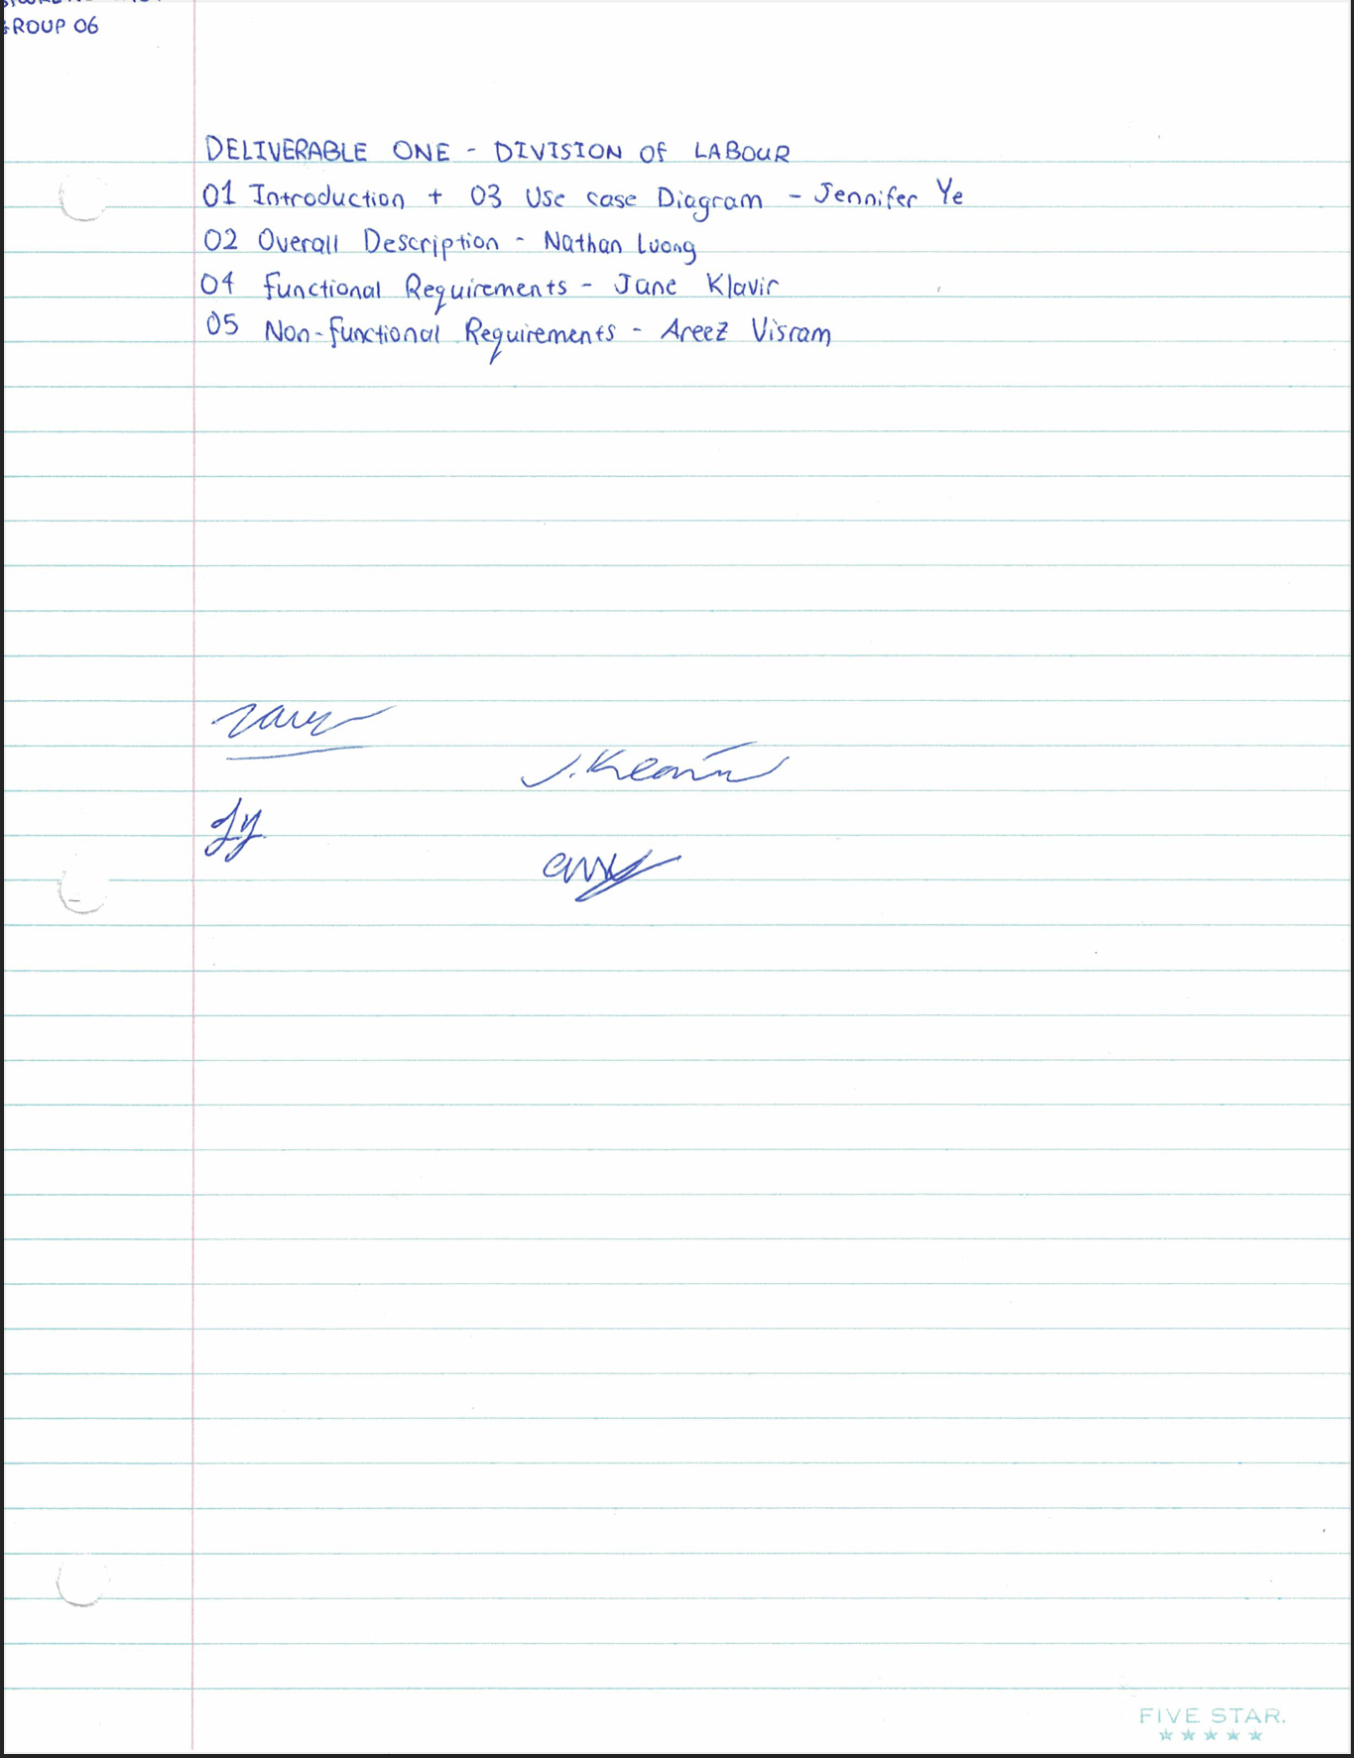
\includegraphics[scale=0.75]{division_of_labour.png}
% End Section

\section{Creative Features}
\label{sec:creative_features}
% Begin Section
Below is a list of creative/innovative features that were brainstormed by the team. The features that were ultimately chosen for implementation are bolded.
\begin{itemize}
	\item Friends (preferred to carpool with friends)
	\item Pre-book (pre book carpools with others for big events)
	\item \textbf{Prompts + social games in the car (add preferences on what kind of level of socialness you want)} 
	\item Emergency button (calls 911 automatically when pressed)
	\item In app payments (integrate with PSP's) 

\end{itemize}
% End Section
\end{document}
%------------------------------------------------------------------------------